%%%%% Literature Review %%%%%
\section{Literature Review} 
This is the Literature Review of the final report.
\subsection{Introduction}
Continuum robots has emerged and attracted a lot of attention since 2008 \cite{review_2008}. Compared with traditional rigid 
joint manipulator, continuum robots stand out for their flexible, highly bendable structure and extremely flexible motion 
performance. This new kind of robot not only changes the code of traditional robot design but also demonstrates unprecedented 
application potential in fields such as medical science \cite{CR_medical_application}. Meanwhile, rigid-flexible-
soft coupled continuum robots combine the multiple advantages of the stability of rigid structures, the flexibility of flexible 
structures, and the compliance of soft structures, and are one of the most promising robots for increasingly complex tasks 
\cite{fishboneCR}. \\
During the development process of robotic science, the limitations of rigid joint robots have gradually shown up, especially 
in applications requiring highly detailed operation and in complex or space-limited environments. With unique bionic structure 
and motion characteristics, continuum robots provide new possibilities to solve these challenges. \\
This paper will discuss different types of existing continuum robots and their working principles, advantages, and disadvantages, 
then propose a proper continuum robot design that can be mainly applied to medical FUS applications.
\subsection{Working Principles}
Continuum robot can be broadly divided into two parts: a continuous bending structure and a fixed base containing actuating and 
controlling devices.\\
The continuous bending structure can be seen as the working arm of the robot. A flexible backbone shapes the arm, and it can be rotated 
and bent by dragging/releasing the different cables (tendons) around it. 
When the joystick in the fixed base is manipulated manually, the programmed stepper motor will step forward/backward by the 
corresponding number of steps. These motors are connected to different cables located in the bending structure (arm), the motors 
dragging the cables, thereby making cable contract. Finally, the contraction of different cables will rotate and bend the backbone, 
which is the core component of the arm, thereby changing the posture of the arm.\\
This process can be likened to the movement of the human arms. cables can be understood as tendons/muscle bundles and backbone as 
the main skeleton.
\begin{figure}[H] %[H] "corresponds to start the figure Here" 
    \centering %alignment can be flushleft or flushright
    \captionsetup{labelsep=colon}
    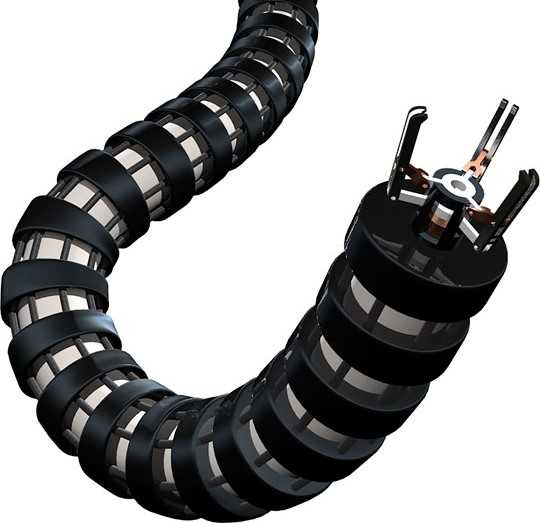
\includegraphics[width=.8\textwidth]{Image/LR/CR_example.jpg} 
    \caption[An example of continuum robot]
    {\centering \textit{\textbf{An example of continuum robot }}\cite{CR_example}.}
    \label{fig:CR_example}
\end{figure}
\noindent Different types of continuum robots have different backbones, actuating and flexible components, but they are generally all 
work under the same working principle stated above. \\
\subsection{Types of Continuum Robots}
Nowadays, a variety of continuum robots exist, each exhibiting unique structures and functions. They serve in different fields 
such as medicine, construction, and exploration. In this section, some of the most popular continuum robots will be introduced, 
providing basic insights into their structures as well as discussing their merits and drawbacks. \\
\subsubsection{Tendon-Driven Robots}
The arm of the Tendon-Driven robot consists of a backbone, several tendons and disks. The backbone defines the structure and 
posture of the entire robot arm, while disks define the diameter and divide the robot arm into segments, and tendons are 
stretched to create deformation and movements of different directions for the robot arm. \\
\begin{figure}[H] %[H] "corresponds to start the figure Here" 
    \centering %alignment can be flushleft or flushright
    \captionsetup{labelsep=colon}
    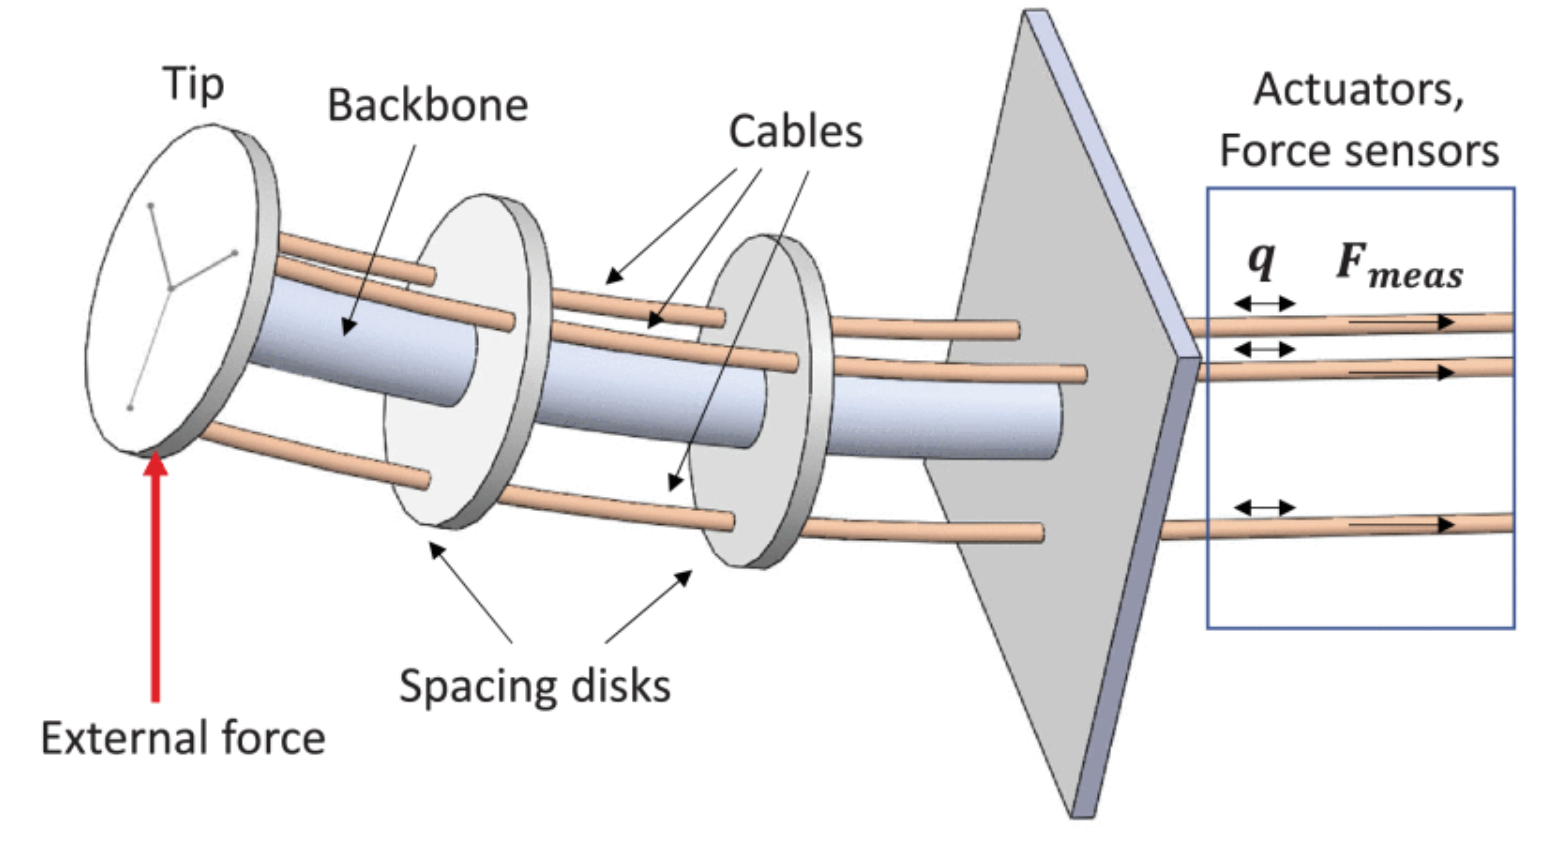
\includegraphics[width=.9\textwidth]{Image/LR/3tendon_1segment_CR.PNG} 
    \caption[The three tendons continuum robot with one segment]
    {\centering \textit{\textbf{The three tendons continuum robot with one segment}} \cite{3tendon_1segment_CR}.}
    \label{fig:3tendon_1segment_CR}
\end{figure}
\noindent Figure \ref{fig:3tendon_1segment_CR} shows only the simplest tenon-driven robots. In practical applications, there 
may be more than one backbone, and the disks are not necessarily parallel. \\
Compared with other continuum robots, one of the most significant advantages of tendon-driven robots is their flexibility. 
This advantage makes it more effective in performing tasks in complex and restrictive Spaces. In addition, due to the simple 
components needed to construct the robot, it is easier to meet lightweight design specifications. Moreover, like the 
concentric-tube continuum robots, tendon-driven continuum robots can be built designed on a small scale with diameters of 
below 10mm \cite{amanov2021tendon}. \\
However, due to its simple actuating principle, more complex algorithms are needed to control it more accurately. Also, the 
tendon-driven robots actuate by pulling the tendon, which makes the friction between the tendon and other components inevitable, 
which will accelerate the wearing speed of the tendon-driven robots.
\subsubsection{Fishbone Robots}
The fishbone robots are inspired by fishbones. It is comprised of multiple "fishbone units" which consist of rigid cross-shaped 
plates and soft rubber sleeves, with a layer of manganese alloy steel elastic plate embedded in the middle to form a rigid-soft 
coupled structure\cite{fishboneCR}. In contract to the existing single-backbone continuum robots, the middle backbone of the 
continuum robot is serially formed by multiple cross- arranged bioinspired fishbone units.  The fishbone units stack layer by 
layer, forming a spine-like shaper. Like tendon-driven robots, it utilizes cables to simulate muscle movement, causing layers 
of fishbones to bend in corresponding directions through cable stretching at different positions. 
\begin{figure}[H] %[H] "corresponds to start the figure Here" 
    \centering %alignment can be flushleft or flushright
    \captionsetup{labelsep=colon}
    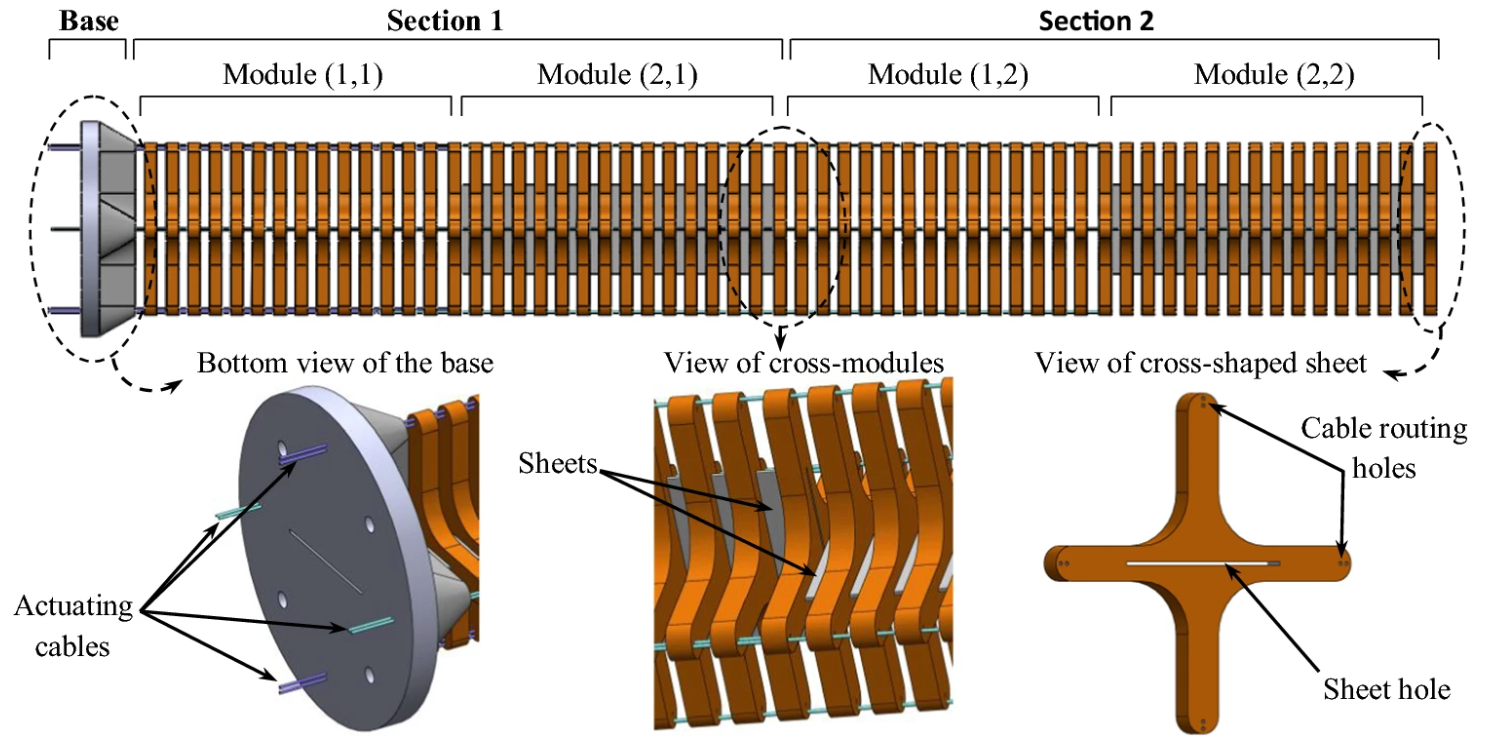
\includegraphics[width=.9\textwidth]{Image/LR/fishbone_CR_amouri2023bio.PNG} 
    \caption[The cable-driven fish bone continuum robot]
    {\centering \textit{\textbf{The cable-driven fish bone continuum robot with cable arrangement}} \cite{amouri2023bio}.}
    \label{fig:fishboneCR_2023bio}
\end{figure}
\noindent Because many fishbone units are stacked together as the backbone of the fishbone continuum robots, the structural 
stability of this kind of robot is very strong. The disadvantage, however, is that it is difficult to make lightweight designs 
since the density of the components is high.
\subsubsection{Concentric Tube Continuum Robots}
concentric tube robots, shaped like retractable walking sticks, consist of many tubes with decreasing diameters. Each tube is 
nested on top of the previous wider tube.  \\
The concentric robots are made of two parts: tubes and coaxial actuation units. The tubes are the main structural element of 
this robot and act as the backbone. The coaxial actuation unit consists of two motors which are responsible for rotation and 
translation movement respectively. Each tube is actuated by an independent coaxial actuation unit. 
\begin{figure}[H] %[H] "corresponds to start the figure Here" 
    \centering %alignment can be flushleft or flushright
    \captionsetup{labelsep=colon}
    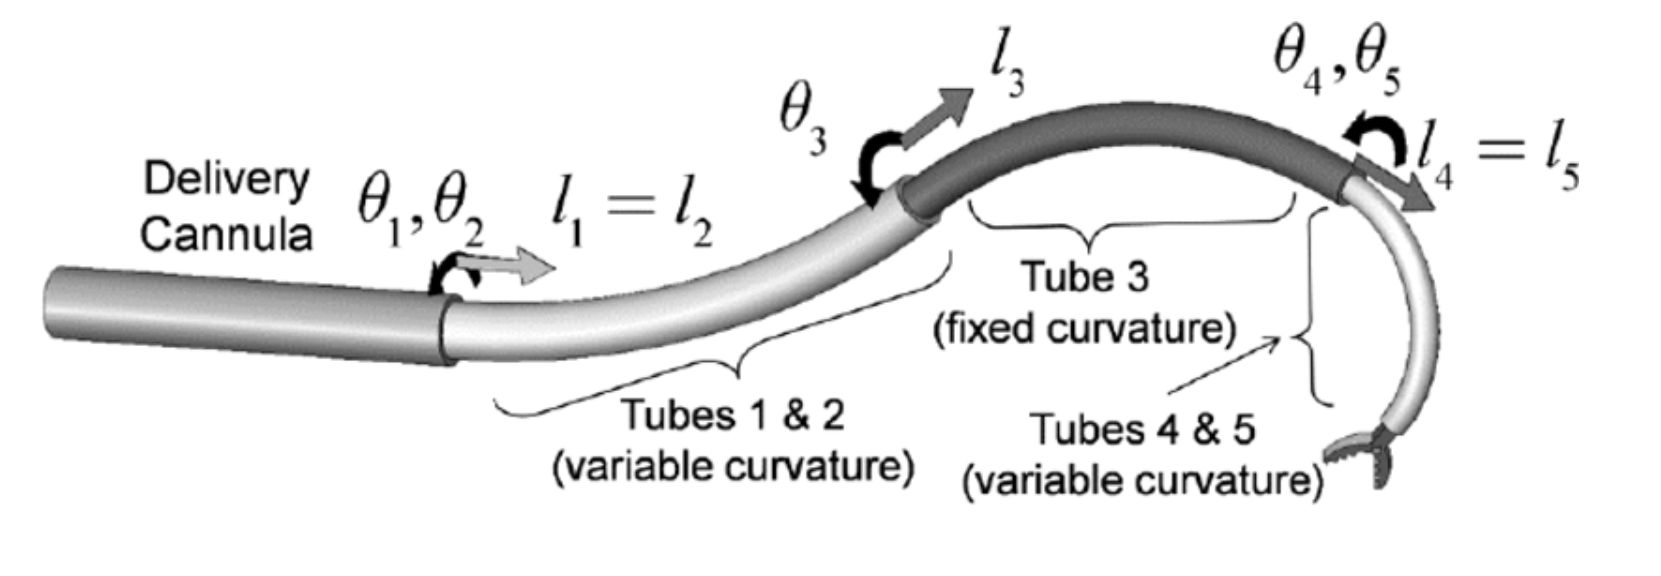
\includegraphics[width=.9\textwidth]{Image/LR/concentric_tube_CR.PNG} 
    \caption[An example concentric tube continuum robot]
    {\centering \textit{\textbf{An example concentric tube continuum robot}} \cite{CTCR_example}.}
    \label{fig:CTCR_example}
\end{figure}
\noindent The most significant advantage of this kind of robots is that of all the continuum robots, concentric tube robots have the 
smallest possible outer diameter and are best suited to work in confined and narrow Spaces. Therefore, it is the ideal choice 
for surgical operations. \\
Their disadvantages, on the other hand, are also very evident. Since each tube requires an independent actuation unit, the 
overall length of the robot cannot be very long, because longer lengths will lead to more tubes, and will lead to more tip 
position errors.



% change to new page
\newpage